\documentclass[twocolumn]{article}

\usepackage[width=17cm,height=22cm]{geometry}
\usepackage[french]{babel}
\usepackage[utf8]{inputenc}
\usepackage{fancyvrb}
\usepackage{authblk}
\usepackage{hyperref}
%% The amssymb package provides various useful mathematical symbols
\usepackage{amssymb}
\usepackage{amsmath}
%% The amsthm package provides extended theorem environments
\usepackage{amsthm}
\usepackage{graphicx}
\usepackage{algorithm}
\usepackage{algorithmic}

\newtheorem{theorem}{Théorème}

\bibliographystyle{alpha}

\title{Optimisation quadratique pour l'apprentissage en ligne d'un bandit contextuel}
\author[1,2]{Emmanuel Daucé}
\author[1]{Hongliang Zhong}
\affil[1]{Ecole Centrale de Marseille, Marseille}
\affil[2]{Institut de Neurosciences des Systèmes, Aix-Marseille Université, Marseille}

\renewcommand\Authands{, et }
\renewcommand\Authand{ et }
\begin{document}
\maketitle

\begin{abstract}
  Nous développons un algorithme d'apprentissage en ligne de classifieurs multiclasses dans le cas où l'information de classification apparaît sous une forme binaire (réponse correcte ou incorrecte). L'absence d'information de label explicite conduit à échantillonner de manière aléatoire l'espace des labels, sur le modèle des bandits contextuels. 
  L'algorithme développé repose  sur l'optimisation à chaque essai d'une fonction de coût, sur le modèle de l'approche ``Passive Agressive'' proposée par \cite{crammer2006online}. 
  L'analyse mathématique permet de mettre en évidence des bornes sur la somme des coûts cumulés, à la fois dans le cas séparable et dans le cas non séparable, comparables aux bornes obtenues dans le cas supervisé. 
  Les expériences numériques confirment le bon comportement de l'algorithme d'apprentissage, à la fois sur des données de grande dimension et sur des jeux de données non-linéairement séparables. 
\end{abstract}

\medskip

\noindent\textbf{Mots-clef}: Optimisation quadratique, Apprentissage en ligne, algorithmes de Bandit, Méthodes à noyaux.

\section{Introduction}
\label{sec:lentete}

Les problèmes de bandit contextuels sont au cœur des problématiques de l’apprentissage automatique. Ils abordent en effet, sous une forme très simple, la question de la recherche \emph{active} de l'information de classification. 

Classiquement, l'apprentissage d'un classifieur repose sur une base d'apprentissage constituée par un ensemble de couples $(x_1,y_1),..., (x_n,y_n)$ où le premier terme du couple est un exemple à classer, généralement représenté sous forme vectorielle,  et le deuxième terme une étiquette indiquant la classe de l'exemple fourni.
L'apprentissage consiste alors à déduire une règle générale de classification à partir de ces exemples, pour pouvoir ensuite classer des exemples inconnus.

Il existe cependant de nombreuses situations d'apprentissage dans lesquelles les étiquettes ne sont pas disponibles telles quelles mais sont un peu ``difficiles'' à obtenir. Nous considérons ici le cas du ``bandit contextuel'' qui est une extension des problèmes de bandit manchot au cas de la classification. 

Un problème de bandit simple est constitué d'une part d'un univers,  d'autre part d'un apprenant. L'univers est constitué d'un ensemble fini de machines à sous numérotées de 1 à $K$. Les machines possèdent des bras. Le comportement des machines est stochastique. Lorsqu'on tire un bras, on obtient un gain $g$ variable selon les machines et selon les tirages. Le gain moyen n'est pas le même sur toutes les machines. Certaines machines offrent en moyenne des gains plus élevés que d'autres. Le but de l'apprenant de maximiser son gain total, ce qui revient à découvrir par expérience la ou les machine(s) offrant l'espérance de gain la plus élevée. Pour trouver cette machine optimale, il faut explorer l'univers, c'est à dire essayer toutes les machines, et plusieurs fois si possible afin de collecter une information plus fiable. Le but d'une expérience est ainsi d'une part d'obtenir un bénéfice maximum, mais également de mieux connaître l'univers pour mieux choisir dans le futur les machines les plus favorables. 

Les problèmes de bandit offrent donc un cadre à l'apprentissage actif, au sens où l'information collectée ne dépend pas uniquement des données présentes dans l'univers, mais également des choix particuliers effectués par l'apprenant. 

Dans ce cadre, on notera un algorithme d'apprentissage selon sa capacité à minimiser le \textit{regret}, qui correspond à l'espérance de la différence entre les gains obtenus à la fin de la partie et le gain qu'on aurait obtenu en appliquant la politique optimale. 
Ainsi, si on considère une séquence de $T$ expériences, le regret se définit comme :
$$R_t = \mathbb{E} \sum_{t=1}^T g_t^* - g_t$$
où $g_t^*$ est le gain obtenu en appliquant la politique optimale et $g_t$ le gain obtenu par l'algorithme d'apprentissage.

Les problèmes de bandit simples se généralisent au cas des bandits dits contextuels \cite{langford2008epoch}. Un problème de bandit contextuel est également défini par un univers et un apprenant. L'univers est constitué par des couples (contexte, distribution). Autrement dit, à chaque contexte distinct correspond une distribution de gains distincte sur l'ensemble des $K$ bras. On peut rajouter une hypothèse supplémentaire selon laquelle à des contextes proches correspondent des distributions proches. Le lien avec les problèmes de classification se fait naturellement en considérant des contextes décrits sur des espaces vectoriels, et des catégories décrites par une distribution de gains sur $K$ bras. Dans le cas que nous considérons, à tout contexte $x$ correspond une étiquette unique $y \in \{1,...,K\}$. Autrement dit, en présence de l'exemple $x$, choisir le bras $y$ apporte un gain positif ($g=1$). Pour tout autre choix, le gain est nul ($g=0$). Une expérience consiste ici, en présence du contexte $x$, à choisir une réponse $\tilde{y} \in \{1,...,K\}$. Si $\tilde{y} = y$, le gain vaut 1 sinon il vaut 0. On note $\mathbf{1}_{\tilde{y} = y}$ le gain obtenu dans le cadre de cette expérience. 

Le lien entre ce problème et les problèmes de classification linéaire a été proposé par Kakade \cite{kakade2008efficient}. Dans le cas de la classification linéaire, des hyperplans séparateurs $w_1, ..., w_K$ définissent les frontières entre les différentes classes dans l'espace des exemplaires.  
Si $x$ est un exemplaire, $\langle w_1, x \rangle > 0$ signifie que $x$ appartient à la classe 1, et $\langle w_1, x \rangle < 0$ qu'il n'appartient pas à la classe 1. Si $x$ est un exemplaire inconnu, on définit généralement la réponse du classifieur comme~:
$$\hat{y} = \arg \max_{k \in\{1,..,K\}}  \langle w_k, x \rangle$$
 
Dans le cadre de l'algorithme ``Banditron'', Kakade propose donc d'apprendre ces hyperplans séparateurs en utilisant un algorithme inspiré du perceptron multiclasse. Il se donne un ensemble de $K$ hyperplans $W_0 = (w^{(1)}_0$, ..., $w^{(K)}_0)$ initialement des vecteurs nuls. A chaque essai, un contexte $x_t$ est lu. Le choix du bras repose sur un tirage aléatoire défini selon~ : $P(\tilde{Y}=k) = (1 - \varepsilon) \mathbf{1}_{k = \hat{y}} + \frac{\varepsilon}{K} $ avec $\varepsilon \in [0,1]$ le paramètre d'exploration. On note $\tilde{y}_t$ le résultat du tirage à l'essai $t$. La mise à jour s'effectue selon~:
$$ W_t = W_{t-1} + \frac{\mathbf{1}_{\tilde{y}_t = y_t} \Phi(x_t,\tilde{y}_t)}{P(\tilde{Y}=\tilde{y}_t)} - \Phi(x_t,\hat{y}_t)$$   
avec $\Phi(x_t,k) = (0, ..., 0,  x_t, 0, .., 0)$ une séquence de vecteurs nuls, excepté à la position $k$ où l'on trouve l'exemplaire $x_t$. Kakade montre que son algorithme converge en espérance vers le classifieur du perceptron, et obtient des garanties sur les bornes d'erreur de son algorithme. 

Toujours dans le cadre des classifieurs linéaires, plusieurs algorithmes d'apprentissage de bandits contextuels ont été proposés dans la littérature. Dans nos expérimentations numériques, nous considérerons également ici l'algorithme ``Confidit'' proposé par Crammer et Gentile \cite{crammer2013multiclass}, reposant sur le perceptron d'ordre 2 et l'exploration non stochastique basée sur le principe UCB \cite{lai1985asymptotically}, et présentant des profils de convergence plus favorables que le Banditron. 


Dans le cas linéairement séparable, l'apprentissage en ligne d'un perceptron multi-classes peut être significativement accéléré en utilisant les principes de l'optimisation quadratique tels que proposés par Vapnik \cite{vapnik1998statistical}. Dans un article récent, Crammer et al \cite{crammer2006online} proposent une méthode d'apprentissage en ligne supervisée reposant sur l'optimisation locale de la fonction de perte ``hinge loss'' définie dans le cadre multi-classe comme : 
$$
	 l_t =[\mathbf{1}_{\hat{y}_t\neq y_t} + \langle W_{t-1}, \Phi(x_t,\hat{y}_t)- \Phi(x_t,y_t)\rangle]_+ 
$$
où $[.]_+$ retourne l'identité pour les valeurs positives et 0 pour les valeurs négatives. 

La résolution du problème :
$$W_{t} = \arg \min_W \frac{1}{2} \| W - W_{t-1}\|^2 + C \xi^2 \hbox{ s.t. } l_t \leq \xi$$
où $C$ correspond au paramètre de raideur, conduit à la mise à jour~:
$$W_{t} =  W_{t-1} + \frac{l_t}{2\|x_t\|^2 + \frac{1}{2C}} (\Phi(x_t,y_t) - \Phi(x_t,\hat{y}_t))$$
Crammer montre que dans le cas linéairement séparable, la somme des pertes au carré est bornée (ce qui est comparable au perceptron). Mais, de manière plus intéressante, il montre également que le regret est  borné en $O(\sqrt{(T)})$ dans le cas non séparable.  

\section{Notre approche}

\subsection{Principe}
L'approche adoptée dans le cadre de cet article est une généralisation assez directe des principes d'optimisation quadratique en ligne proposés par Crammer au cas des bandits contextuels. Cette extension nécessite de définir une fonction de perte spécifique. 

Soit un classifieur linéaire défini à l'essai $t$ par le jeu de paramètres $W_{t-1}$. Après avoir observé l'exemplaire $x_t$, le choix $\tilde{y}_t$ repose sur un tirage selon la distribution: $$P(\tilde{Y}=k) = (1 - \varepsilon) \mathbf{1}_{k = \hat{y}} + \frac{\varepsilon}{K} $$ avec $\varepsilon \in [0,1]$ le paramètre d'exploration, et $\hat{y}$ la catégorie correspondant au meilleur score des produits salaires entre entre l'exemplaire et les différentes séparatrices.  

Après avoir émis la proposition $\tilde{y}_t$, l'apprenant reçoit un gain $g_t$ égal à 1 si la catégorie proposée est correcte et 0 sinon, soit $g_t = \mathbf{1}_{\tilde{y}_t=y_t}$. 

La perte instantanée est ici définie comme :
$$l_t = [1 + (1 - 2 g_t) \langle W_{t-1}, \Phi(x_t,\tilde{y}_t)\rangle]_+$$
autrement dit~:
\begin{itemize}
	\item[] $l_t = [1 - \langle W_{t-1}, \Phi(x_t,\tilde{y}_t)\rangle]_+$ si $g_t=1$;
	\item[] $l_t = [1 + \langle W_{t-1}, \Phi(x_t,\tilde{y}_t)\rangle]_+$ sinon
\end{itemize}
Dans le premier cas (le choix est correct), la perte décroît avec $\langle W_{t-1}, \Phi(x_t,\tilde{y}_t)\rangle$ jusqu'à 0. Au contraire, dans le second cas (choix incorrect), la perte augmente avec le produit $\langle W_{t-1}, \Phi(x_t,\tilde{y}_t)\rangle$.
Minimiser la perte revient donc à faire croître le produit $\langle W_{t-1}, \Phi(x_t,\tilde{y}_t)\rangle$ dans le premier cas, et à faire décroître le produit $\langle W_{t-1}, \Phi(x_t,\tilde{y}_t)\rangle$  dans le second cas.

La résolution du problème d'optimisation suivant~:
$$W_{t} = \arg \min_W \frac{1}{2} \| W - W_{t-1}\|^2 + C \xi^2 \hbox{ s.t. } l_t \leq \xi$$
où $C$ correspond au paramètre de raideur, conduit à la mise à jour~:
$$W_{t} =  W_{t-1} + \frac{l_t}{\|x_t\|^2 + \frac{1}{2C}} (2g_t - 1) \Phi(x_t,\tilde{y}_t)$$
(voir \cite{crammer2006online} pour plus de détails)
%\paragraph{Bandit Passive-Aggressive (BPA)}
	%\caption{BPA}
\begin{algorithm}
	\caption{Bandit Passive Aggressive (BPA)}\label{algo:BPA}
	\begin{algorithmic}
		\STATE $\ \ $
		\STATE paramètres:  $\varepsilon$, $C$.
		\STATE $W_0 \leftarrow 0$ (vecteur nul)
		\FOR {$t$ = 1,\dots, $T$}
		\STATE Lire $x_t$.
		\STATE Etablir $\hat{y}_t = \underset{i = 1,\dots,K}{\text{argmax}}\left\langle W_{t-1} ,\Phi(x_t,i)\right\rangle$
		\FOR {$i = 1,...,K$}
		\STATE $p_{i,t}\leftarrow (1-\varepsilon)\mathbf{1}_{i = \hat{y}_t} + \frac{\varepsilon}{K}$
		\ENDFOR
		\STATE Choisir aléatoirement $\tilde{y}_t$ selon $p_t = \left(p_{1,t},\dots ,p_{K,t}\right)$
		\STATE Lire $g_t = \mathbf{1}_{(\tilde{y}_t=y_t)}$
		\STATE $l_t \leftarrow [ 1+(1-2g_t)\left\langle W_{t-1},\Phi(x_t,\tilde{y}_t)\right\rangle]_{+}$ 
		\STATE $W_t \leftarrow W_{t-1} + (2g_t-1)\frac{l_t}{\parallel\Phi(x_t,\tilde{y}_t)\parallel^2 + \frac{1}{2C}}\cdot\Phi(x_t,\tilde{y}_t)$
		\ENDFOR
	\end{algorithmic}
\end{algorithm}

\subsection{Analyse}
Soit $U$ est un classifieur quelconque de l'espace des classifieurs, on note $l_t^{\ast}$ la perte obtenue par ce classifieur à l'instant $t$. On démontre les deux théorèmes suivants (en négligeant la constante de raideur, soit $C\rightarrow \infty$, pour simplifier) :

\begin{theorem}
	\label{theo:BPAT1}
	Soit $(x_1,y_1),...,(x_T,y_T)$ une séquence d'exemples linéairement séparables où $x_t \in \mathbb{R}^d$, $y_t\in \{1,...,K\}$ et $\parallel x_t \parallel\leqslant R$ pour tout $t$, et $U \in \mathbb{R}^{K\times d}$ tel que $ \forall t, l^*_t=0$. Alors, la perte au carré cumulée de l'algorithme \ref{algo:BPA} est bornée par:
	\begin{equation}
	\sum_{t=1}^{T} l_t^2 \leqslant R^2\cdot \parallel{U}\parallel^2
	\end{equation}
\end{theorem}

\begin{proof}
	Soit $\Delta_t$ telle que:
	\[\Delta_t = \parallel{W_{t-1}-U}\parallel^2-\parallel{W_t-U}\parallel^2\]
	La somme de 1 à $T$ des $\Delta_t$  se réduit à:
	\begin{align}
    \sum_{t=1}^{T}\Delta_t &= \sum_{t=1}^{T} \left( \parallel{W_{t-1} - U}\parallel^2-\parallel{W_t - U}\parallel^2 \right)\nonumber\\ 
    &= \parallel{W_0 - U}\parallel^2-\parallel{W_T-U}\parallel^2\nonumber
	\end{align}	
	Sachant que $W_0 = \vec{0}$, 
	\begin{equation}
	\label{equa:delta}
	\sum_{t=1}^{T}\Delta_t = \parallel{U}\parallel^2 - \parallel{W_T-U}\parallel^2 \leqslant \parallel{U}\parallel^2 
	\end{equation}
	
	En utilisant la définition de la mise à jour~: %in Eq.\ref{eq:,
	\begin{align}
	\Delta_t =& -2\left\langle (W_{t-1} - U), (2g_t-1)\frac{l_t}{\parallel{x_t}\parallel^2}\Phi(x_t,\tilde{y}_t)\right\rangle \nonumber\\
	&- \left\| \frac{l_t}{\parallel{x_t}\parallel^2}\Phi(x_t,\tilde{y}_t)\right\|^2
	\nonumber
	\end{align}
	%With    and   ,
	et en remarquant que~:
	\begin{itemize}
		\item[] $l_t = [1+(1-2g_t)\langle W_{t-1},\Phi(x_t,\tilde{y}_t)\rangle]_+$
		\item[] $l_t^{\ast} = [1+(1-2g_t)\langle U,\Phi(x_t,\tilde{y}_t)\rangle]_+$
		\item[] $\parallel{\Phi(x_t,\tilde{y}_t)}\parallel = \parallel x_t\parallel$
	\end{itemize}
	on obtient:
	\begin{align}
	\Delta_t =& 2l_t\frac{(1-2g_t)\langle W_{t-1}, \Phi(x_t,\tilde{y}_t)\rangle - (1-2g_t)\langle U, \Phi(x_t,\tilde{y}_t)\rangle}{\|x_t\|^2} \nonumber\\
	&-\left( \frac{l_t}{\parallel{x_t}\parallel^2}\parallel{\Phi(x_t,\tilde{y}_t)}\parallel \right)^2\nonumber
	\end{align}
	Sachant que $\Delta_t = 0$ quand $l_t = 0$, et $l^*_t \geq  1+(1-2g_t)\cdot\langle U,\Phi(x_t,\tilde{y}_t)\rangle$, on obtient : 
	\begin{align}
	\Delta_t\geqslant& 2l_t\frac{l_t - l_t^{\ast}}{\parallel{x_t}\parallel^2}-\left( \frac{l_t}{\parallel{x_t}\parallel^2}\parallel x_t\parallel \right)^2\nonumber\\
	=& \frac{l_t^2-2l_t l_t^{\ast}}{\parallel x_t\parallel^2}\nonumber
	\end{align}
Sachant que $U$ est tel que $\forall t \in [1,...,T]$ , $l_t^{\ast} = 0$ ,
	%, following the Eq.~\ref{sumDelta},
	
	\[\Rightarrow \parallel{U}\parallel^2 \geqslant \sum_{t=1}^{T}\Delta_t \geqslant \sum_{t=1}^{T}  \frac{l_t^2}{\parallel{x_t}\parallel^2}
	\geqslant 
	\sum_{t=1}^{T}  \frac{l_t^2}{R^2}
	\]
	\[\Rightarrow\sum_{t=1}^{T} l_t^2 \leqslant R^2 \cdot \parallel{U}\parallel^2\]
\end{proof}
\begin{theorem}
	\label{theo:BPAT2}
	Soit $(x_1,y_1),...,(x_T,y_T) $ une séquence d'exemples telle que   $x_t\in \mathbb{R}^d$, $y_t \in \{1,...,K\}$ et $\parallel{x_t}\parallel \leqslant R$ pour tout $t$. Alors, quel que soit  $U \in \mathbb{R}^{K\times d}$, la perte a carré cumulée de  l'algorithme \ref{algo:BPA} est bornée par:
	\[\sum_{t=1}^{T}l_t^2 \leqslant \left(R\parallel{U}\parallel+2 \sqrt{\sum_{t=1}^{T}(l_t^{\ast})^2}\right)^2 \]
\end{theorem}
\begin{proof}
	Un résultat intermédiaire du théorème \ref{theo:BPAT1} indique que: 
	\[\sum_{t=1}^{T}l_t^2 \leqslant R^2\cdot \parallel{U}\parallel^2 + 2\sum_{t=1}^{T}l_t l_t^{\ast}\]
	Pour borner la partie droite de l'inégalité, on note $A_t = \sqrt{\sum_{t=1}^{T}l_t^2}$ et $B_t = \sqrt{\sum_{t=1}^{T}(l_t^{\ast})^2}$, 
	\begin{align}
	2(A_tB_t)^2-2(\sum_{t=1}^{T}l_tl_t^{\ast})^2 =& \sum_{i=1}^{T}\sum_{j=1}^{T}l_i^2(l_j^{\ast})^2+\sum_{i=1}^{T}\sum_{j=1}^{T}l_j^2(l_i^{\ast})^2 \nonumber\\
	&- 2\sum_{i=1}^{T}\sum_{j=1}^{T}l_il_jl_i^{\ast}l_j^{\ast}\nonumber\\
	=& \sum_{i=1}^{T}\sum_{j=1}^{T}(l_il_j^{\ast}-l_jl_i^{\ast})^2 \geqslant 0 \nonumber
	\end{align}
	
	\begin{align}
	\sum_{t=1}^{T}l_t^2 \leqslant R^2 \cdot \parallel{U}\parallel^2+2\sum_{t=1}^{T}l_tl_t^{\ast}\leqslant R^2 \cdot \parallel{U}\parallel^2+2A_tB_t\nonumber
	\end{align}
	puis, sachant que~:
	\[A_t^2 -2 A_tB_t+B_t^2\leqslant R^2\parallel{U}\parallel^2+B_t^2\]
	on obtient~:
	\[A_t \leqslant B_t+\sqrt{R^2\parallel{U}\parallel^2+B_t^2}\]
	et en utilisant le fait que~: $\sqrt{a+b}\leqslant \sqrt{a}+\sqrt{b}$,
	\[A_t \leqslant R\parallel{U}\parallel+2 B_t\]
	on obtient~:
	\[\sum_{t=1}^{T}l_t^2 \leqslant \left(R\parallel{U}\parallel+2 \sqrt{\sum_{t=1}^{T}(l_t^{\ast})^2}\right)^2 \]
\end{proof}

%Pour les affiliations, vous pouvez utiliser
%\href{http://ctan.org/pkg/authblk}{le paquet \texttt{authblk}}.

Les bornes obtenues ici sont comparables  à celles obtenues par Crammer dans le cadre de la classification supervisée  \cite{crammer2006online}. Il est à noter que la prise en compte du terme de régularisation $C$ devrait permettre, sous certaines conditions, d'atteindre  un regret de l'ordre de $O(\sqrt{T})$ dans le cas non-linéairement séparable (ce résultat n'est pas développé ici). Il est par ailleurs remarquable de constater que les garanties de convergences de notre algorithme sont les mêmes que dans le cas supervisé, étant donnée la moindre information utilisée et le caractère stochastique de la fonction de décision. On notera néanmoins le caractère plus ``faible'' de la fonction de perte utilisée, de sorte que nos résultats ne garantissent pas que la bonne réponse sera atteinte, mais seulement que la mauvaise réponse ne sera pas atteinte.

\subsection{Extensions}
Le plongement des données d'entrée dans des espaces de Hilbert à noyaux reproduisants (RKHS) permet d'étendre notre approche aux jeux de données non linéairement séparables. 

Soit $\mathcal{H}$ un espace de Hilbert à noyaux reproduisants dont le produit scalaire est défini à l'aide de la fonction noyau $\mathcal{K}$. On note $\mathcal{K}(x,.)$ la projection de l'exemplaire $x$ dans $\mathcal{H}$, avec $\forall f \in \mathcal{H}, \langle f,\mathcal{K}(x,.)\rangle_\mathcal{H} = f(x) $.
 

Le classifieur est dans ce cadre défini comme un ensemble de fonctions : $\mathcal{F} = \{f^{(1)}, ..., f^{(K)}\}$ avec :
$$\hat{y} = \arg \max_k f^{(k)}(x)$$

Soit $\mathcal{F}_0=\{0, ..., 0\}$ le classifieur initial. A chaque essai, il est mis à jour selon la règle définie précédemment, soit à l'instant $t$~:
$$\mathcal{F}_t = \{f^{(1)}_t, ..., f^{(K)}_t\}$$
$$\forall k, f^{(k)}_t = \sum_{t^\prime = 1} ^t  \frac {\mathbf{1}_{k=\tilde{y}_{t^\prime}}l_{t^\prime}}{\mathcal{K}(x_{t^\prime},x_{t^\prime})+\frac{1}{2C}} (2g_{t^\prime} - 1)\mathcal{K}(x_{t^\prime},.)$$
$$ l_t = [1 + (1-2g_t) f_{t-1}^{(\tilde{y}_t)}(x_t)]_+$$

En notant $\alpha_t^{(k)} = \frac {\mathbf{1}_{k=\tilde{y}_{t}}l_{t}}{\mathcal{K}(x_{t},x_{t})+\frac{1}{2C}} (2g_{t} - 1)$, il vient :
$$\forall k, f^{(k)}_t = \sum_{t^\prime = 1} ^t \alpha_{t^\prime}^{(k)} \mathcal{K}(x_{t^\prime},.)$$

Autrement dit chaque séparatrice $f^{(k)}$ est définie par un ensemble de vecteurs supports ($x_{t_1^{(k)}}$, ..., $x_{t_i^{(k)}}$, ...  ) tels que $\forall i, \alpha_{t_i^{(k)}}^{(k)} \neq 0$.


Le nombre de vecteurs supports augmente de 1 chaque fois que la perte est non nulle. De par le théorème 1, nous savons que ce nombre est borné dès lors que les données sont séparables dans l'espace de redescription. 

Afin de contrôler plus strictement le nombre de vecteurs supports, nous considérons une approche alternative basée sur la minimisation du risque régularisé par descente de gradient comme proposé dans \cite{kivinen2004online}~:
$$R(\mathcal{F}) = \mathbb{E}\left[ l_t + \frac{\lambda}{2}\|\mathcal{F}\|^2_\mathcal{H}\right]$$
On obtient dans ce cas la règle de mise à jour~:
$$f_t^{(k)}=\left\{
\begin{array}{l}
(1-\eta\lambda) f_{t-1}^{(k)} + \eta (2g_t-1) \mathcal{K}(x_t,.) \text{ si } k=\tilde{y}_t\\
 f_{t-1}^{(k)} \text{ sinon}
\end{array}
\right.
$$
avec $\eta$ paramètre d'apprentissage et $\lambda$ paramètre de régularisation. En notant 
$$\sigma_t^{(k)} = \sum_{t^\prime=1}^t
\mathbf{1}_{\tilde{y}_{t^\prime}=k}$$
on obtient dans ce cas:
$$\forall k, f^{(k)}_t = \sum_{t^\prime = 1} ^t \alpha_{t^\prime}^{(k)} \mathcal{K}(x_{t^\prime},.)$$
et
$$\alpha_{t^\prime}^{(k)} = \mathbf{1}_{\tilde{y}_{t^\prime}=k}(1 - \eta \lambda)^{\sigma_t^{(k)} - \sigma_{t^\prime}^{(k)}-1}  \eta (2g_{t^\prime}-1)$$

Comme proposé par Kivinen, il suffit alors de tronquer la séquence de vecteurs supports servant à définir la séparatrice en éliminant les termes les plus faibles, typiquement les exemplaires $t^\prime$ tels que $\sigma_{t^\prime}^{(k)} > H$, avec $H$ horizon définissant le nombre maximal de vecteurs supports conservés par séparatrice. Cet artifice borne naturellement le nombre de vecteurs supports du classifieur, en ne considérant que les exemplaires les plus récemment observés (les exemplaires les plus anciens sont ``oubliés'').  Kivinen montre que l'erreur de troncature décroît exponentiellement avec la taille de l'horizon choisi. 


  

%Et évidemment, vous ajoutez ensuite les paquets que vous voulez
%utiliser, les macros les définitions de théorèmes etc... Nous
%recommandons le paquet \texttt{hyperref} puisque les documents
%\texttt{PDF} seront en ligne si vous avez donné votre accord.

\section{Expériences}

\subsection{Jeux de données et paramètres}
\label{subsec:BPAE}
Nous évaluons ici notre algorithme à l'aide de deux jeux de données synthétiques et trois jeu de données réels dont les caractéristiques sont fournies dans la table Table~\ref{table:mce}.

\begin{table}[h]
	\caption{Caractéristiques des cinq jeux de données}
	\label{table:mce}
	\begin{center}
		\begin{tabular}{l l l l}
			{\bf Jeu}  & {\bf nb ex.} & {\bf dim.} & {\bf K}\\
			\hline
			SynSep & $10^5$ 	& 400 	& 9 \\
			
			SynNonSep & $10^5$ & 400 	& 9 \\
			
			RCV1-v2  & $10^5$ 	& 47236 	& 53 \\
			
			Pendigits 	& 7494	& 16	& 10	\\
			
			Segment & 2310	& 19	& 7	\\
		\end{tabular}
	\end{center}
\end{table}

\paragraph{Jeux de données}
Les 3 premiers jeux de données testent le comportement de l'algorithme dans le cas de données de grande dimension, c'est à dire pour des données susceptibles de provoquer de l'encombrement mémoire avec les approches d'ordre 2 classiques. Il s'agit typiquement de vecteurs de caractéristiques basés sur l'analyse de textes, dont le nombre de caractéristiques peut avoisiner les 50000.
 
Le premier jeu de données, nommé SynSep, est un jeu de données synthétique linéairement séparable, qui simule de façon simplifiée des données de type document.  Les différentes coordonnées représentent des termes d'un petit vocabulaire de taille $400$. Il est constitué de 9 classes. Le nombre d'exemplaire généré est $10^5$.
La méthode de construction de ce jeu de données peut être trouvées dans \cite{kakade2008efficient}. 

Le second jeu de données, nommé SynNonSep,est construit de la même façon, à l'exception d'un bruit de label à 5\%, ce qui rend le jeu de données non-séparable. 

Le troisième jeu de données provient de la collection Reuters RCV1-v2 \cite{David04RCV}.
Le jeu original est constitué d'instances multi-label. Afin d'obtenir un label par instance, nous effectuons le prétraitement proposé par \cite{RB08a}. Le jeu obtenu est constitué de 53-classes, la dimension des vecteurs est 47236 et le nombre d'instances est $10^5$. 

Les deux derniers jeux de données sont constitués de données réelles, de dimension plus faible, et avec un nombre d'exemplaires également plus faible. Nous comparons dans ce cas différents algorithmes en plongeant les données dans des espaces de fonctions noyaux.  

Le quatrième jeu de données, nommé Pendigits, est un jeu de données réel créé pa E. Alpaydin and F. Alimoglu \cite{alimoglu1996combining}. 
Il contient 7494 instances, avec 16 caractéristiques par instance et 10 classes. 

Le cinquième jeu de données appelé `Segment' \cite{Lichman:2013} contient 2310 instances, chacune d'elle étant un extrait d'images naturelles basé sur des régions de 3x3 pixels, avec 19 caractéristiques et 7 classes. 


%The fourth and fifth data sets are collected from \cite{letter26SC,number10SC}. The fourth data set is to identify each of a large number of black-and-white rectangular pixel displays as one of the 26 capital letters in the English alphabet. The character images were based on 20 different fonts and each letter within these 20 fonts was randomly distorted to produce a file of 20000 unique stimuli. Each stimuli was converted into 16 primitive numerical attributes (statistical moments and edge counts). It forms a 26-class, 16-dimensional real data set of size $20000$. The fifth data set is a digit data base made by collecting 250 samples from 44 writers, using only (x,y) coordinate information represented as constant length feature vectors, which were resampled to 8 points per digit (therefore the data set contains 8 points $\times$ 2 coordinates = 16 features). This one is a 10-class, 16-dimensional real data set of size $10992$.

Les paramètres utilisés dans les différentes simulations sont donnés dans la table 2. Ces paramètres ont été choisis par validation croisée sur le taux de classification final, afin de comparer de manière fiable les différentes méthodes utilisées. 


\begin{table}[h]
	\caption{Paramètres utilisés pour les différents jeux de données. Pour les en-têtes de colonne, P. désigne le Perceptron, PA désigne le Passif Agressif, B désigne le Banditron, C désigne le Confidit, BPA est le Bandit Passif Agressif, KB est le Kernel Banditron, KBPA est le Kernel BPA et KSGD est le gradient stochastique à noyaux. Pour les en-têtes de lignes, SS désigne SynSep, SN SynNonSep, R Reuters, P Pendigits et S Segment.}
	\label{table:bpa}
	\vspace{.3cm}
	\begin{small}
	
	%\begin{center}
	
%		\begin{tabular}{llllll}
%			
%			\hline
%			{\bf }  & {\bf P} & {\bf PA } & {\bf B}& {\bf C} & {\bf BPA}\\
%			\hline
%			SS & $\varnothing$ & $C=0$ & $\varepsilon = 0.014$ &$\eta = 10^3$ & $\varepsilon = 0.4$\\
%			&&&&& $C = \infty$\\
%			
%			SN & $\varnothing$ & $C=10^{-2}$ & $\varepsilon =0.65$ & $\eta = 10^3$& $\varepsilon = 0.8$\\
%			&&&&& $C = 10^{-2}$\\			
%			R & $\varnothing$ & $C=10^{-2}$ & $\varepsilon =0.4$ & $\eta = 10^2$ & $\varepsilon = 0.2$\\
%			&&&&& $C = 10^{-2}$\\
%			\hline
%			&{\bf KB} & {\bf BPA} & {\bf KBPA} &{\bf KSGD}\\
%			\hline
%			P & $\sigma = 1$ & $C = 10^{-2}$ &$\sigma = 1$&$\sigma = 1$\\
%			&&$\varepsilon = 0.2$& $C = 1$ & $H = 500$\\
%			&&& $\varepsilon = 0.2$ &\\
%			S & $\sigma = 10$ & $C = 10^{-2}$ & $\sigma = 10$&$\sigma = 10$\\
%			&&$\varepsilon = 0.2$& $C = 1$& $H = 200$\\
%			&&& $\varepsilon = 0.2$ &
%			%LR(26 letters) & null &  $C=0.1$ & $\varepsilon = 0.2$& $\eta=10^2$ & $\varepsilon = 0.8,C= 1$ \\
%			
%			%LR(10 numbers) & null & $C=0.1$ & $\varepsilon= 0.4$& $\eta = 10$ & $\varepsilon = 0.6,C=1$\\
%			
%		\end{tabular}
		\hspace{-.8cm}
		\begin{tabular}{llllll}
			
			\hline
			{\bf }  & {\bf P} & {\bf PA } & {\bf B}& {\bf C} & {\bf BPA}\\
			\hline
			SS & $\varnothing$ & $C=\infty$ & $\varepsilon = 0.014$ &$\eta = 10^3$ & $\varepsilon = 0.4$\\
			&&&&& $C = \infty$\\
			
			SN & $\varnothing$ & $C=10^{-2}$ & $\varepsilon =0.65$ & $\eta = 10^3$& $\varepsilon = 0.8$\\
			&&&&& $C = 10^{-2}$\\			
			R & $\varnothing$ & $C=10^{-2}$ & $\varepsilon =0.4$ & $\eta = 10^2$ & $\varepsilon = 0.2$\\
			&&&&& $C = 10^{-2}$\\
			\hline
			&{\bf KB} & {\bf BPA} & {\bf KBPA} &{\bf KSGD}\\
			\hline
			P & $\sigma = 10$ & $\varepsilon = 0.3$ &$\sigma = 10$&$\sigma = 10$\\
			&$\varepsilon =0.1$&& $\varepsilon = 0.3$ & $H = 500$\\
			S & $\sigma = 1$ & $\varepsilon = 0.3$ & $\sigma = 1$&$\sigma = 1$\\
			&$\varepsilon =0.1$&&$\varepsilon = 0.3$ & $H = 200$\\
			%LR(26 letters) & null &  $C=0.1$ & $\varepsilon = 0.2$& $\eta=10^2$ & $\varepsilon = 0.8,C= 1$ \\
			
			%LR(10 numbers) & null & $C=0.1$ & $\varepsilon= 0.4$& $\eta = 10$ & $\varepsilon = 0.6,C=1$\\
			
		\end{tabular}
	%\end{center}
	\end{small}
\end{table}

\subsection{Resultats}

Tous les algorithmes comparés sont des algorithmes d'apprentissage en ligne. Le classifieur est donc mis à jour après chaque essai et évolue continuellement au cours de la session d'apprentissage. Chaque exemplaire n'est présenté qu'une seule fois. L'apprentissage du classifieur démarre dès la présentation du premier exemplaire et s'achève après la présentation du dernier exemplaire. Pour chaque exemplaire présenté, on mesure la réussite sous forme d'erreur $\mathbf{1}_{\hat{y}_t\neq y_t}$ ou de perte $l_t$. 

Les algorithmes du Perceptron et Passif-Agressif sont des algorithmes \emph{supervisés}. Ils disposent donc d'une information de classification plus riche que les algorithmes Banditron, Confidit et Bandit Passif-Agressif qui ne disposent que d'une information de type bandit (autrement dit binaire).

Les mesures utilisées pour comparer les algorithmes sont le taux d'erreur cumulé et le taux d'erreur moyen. Le taux d'erreur cumulé se définit à chaque essai $t$ comme le nombre d'erreurs jusqu'à $t$, soit:
$$M_t = \sum_{t'=1}^t \mathbf{1}_{\hat{y}_{t^\prime}\neq y_{t^\prime}} $$
Le taux d'erreur moyen, calculé par fenêtre de 100 essais, permet d'estimer plus précisément l'évolution des performances des algorithmes au cours de l'apprentissage:
$$\forall t>99, \bar{m}_t = \frac{1}{100} \sum_{t'=t - 99}^t \mathbf{1}_{\hat{y}_{t^\prime}\neq y_{t^\prime}}$$
  
Dans le cas du Banditron et du Bandit Passif-Agressif qui utilisent une politique d'exploration $\varepsilon$-glouton, le choix effectif $\tilde{y}_t$ diffère de $\hat{y}_t$ dans une proportion égale à $\varepsilon$. Une erreur résiduelle subsiste donc nécessairement, même lorsque le classifieur sépare correctement les données. Pour l'évaluation, nous considérons l'erreur de classification et non l'erreur effective, autrement dit nous négligeons l'erreur d'exploration des algorithmes de Banditron et de Bandit Passif Agressif, afin de comparer de manière équitable les caractéristiques des classifieurs calculés par les différents algorithmes.

\begin{figure}[ht!]
	\centerline{
		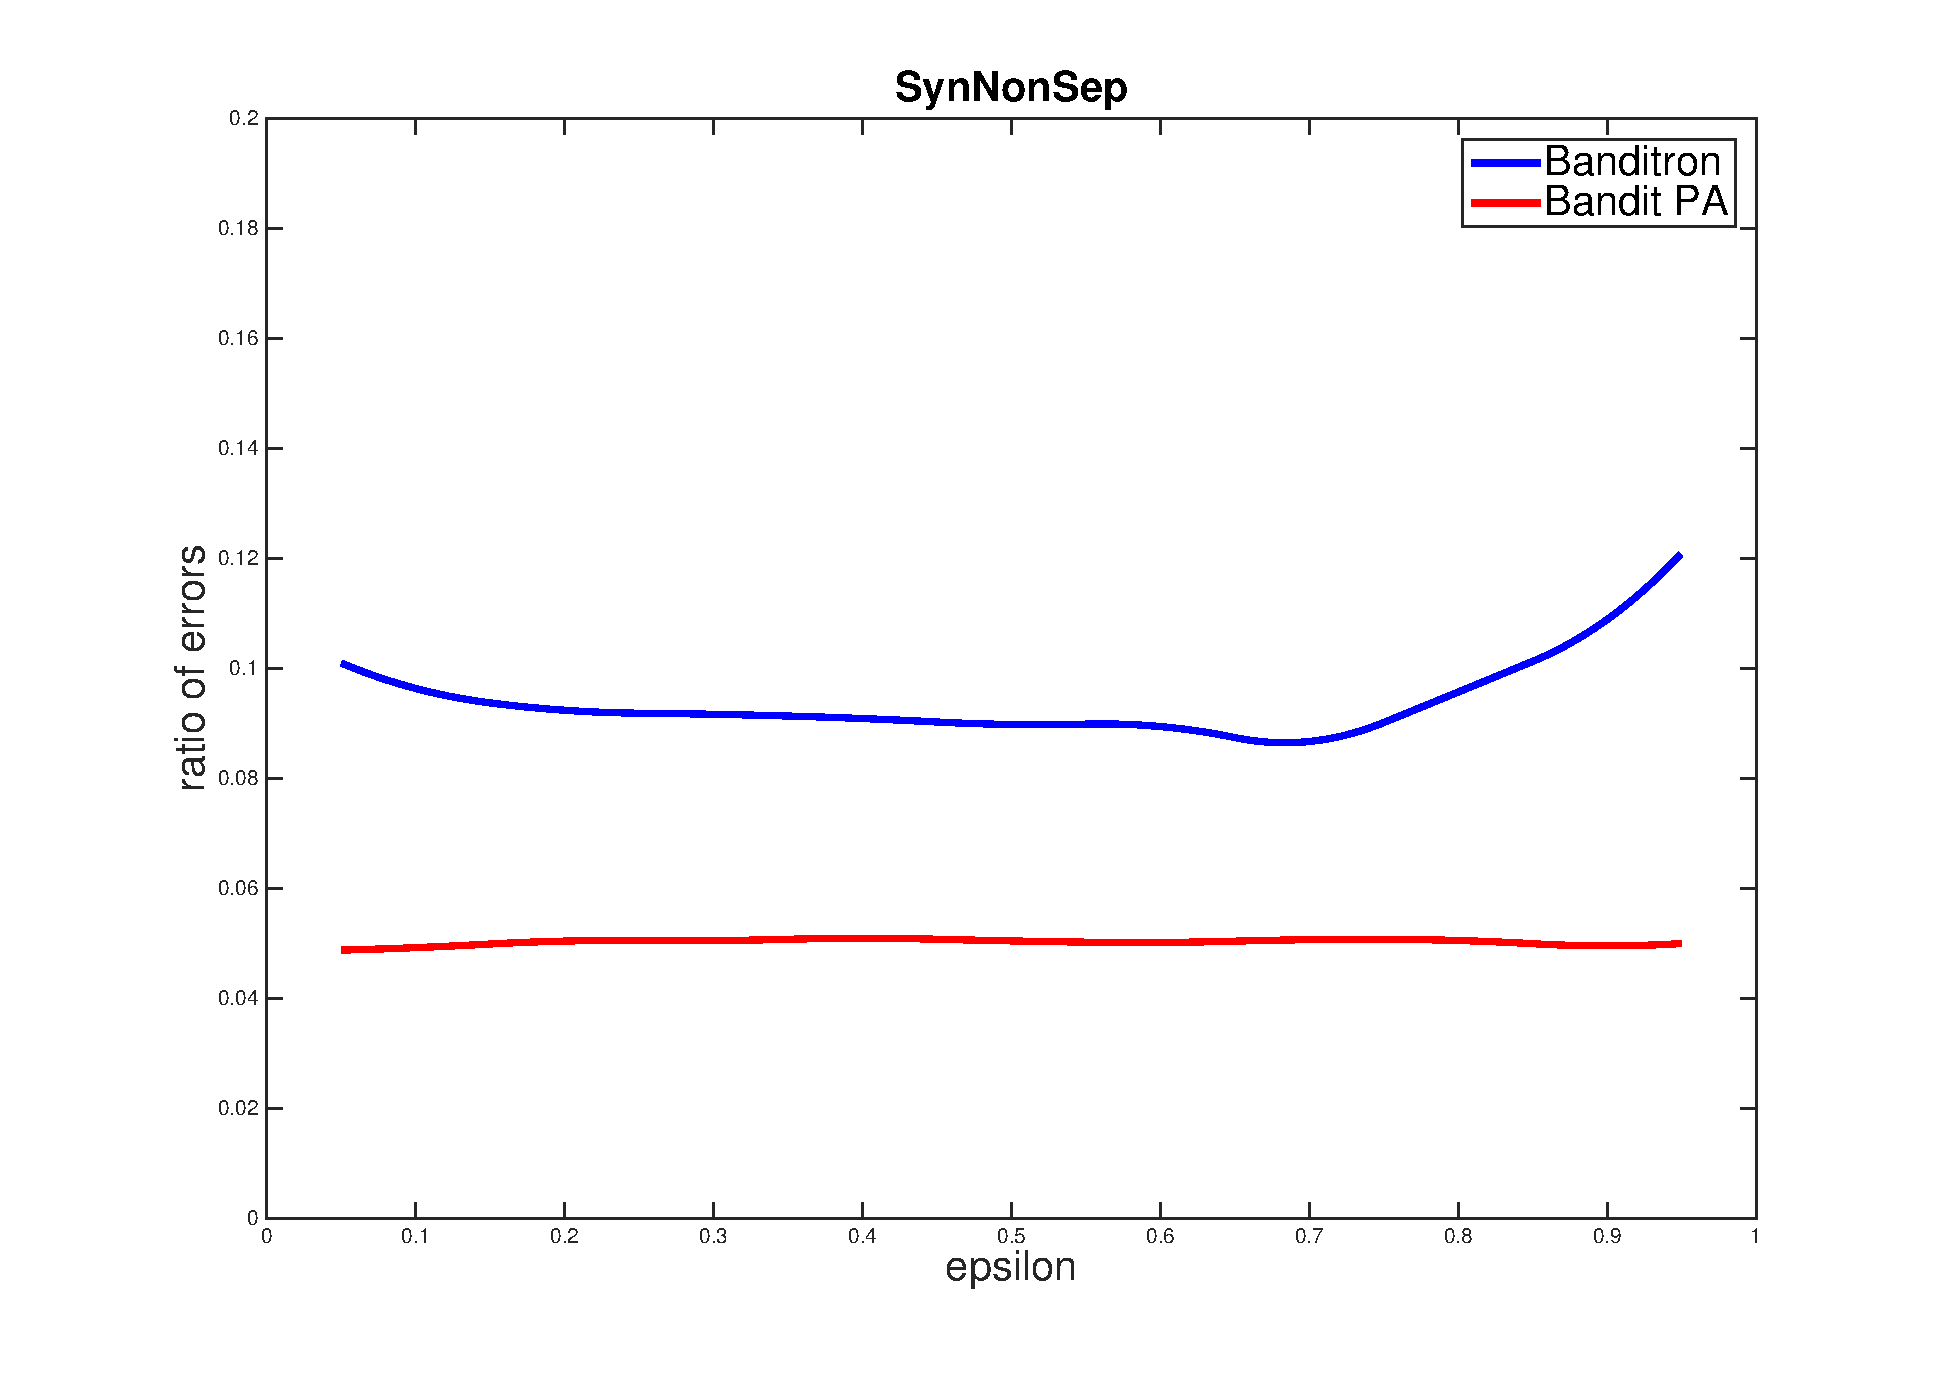
\includegraphics[width=\linewidth]{figs/SynNonSep_gamma.eps}}
	\caption{Taux d'erreur moyen du Banditron et du BPA en fonction du taux d'exploration $\varepsilon$ sur le jeu de données SynNonSep. }
	\label{pic:BPASNSerr}
\end{figure}

\begin{figure}[ht!]
	\centerline{
		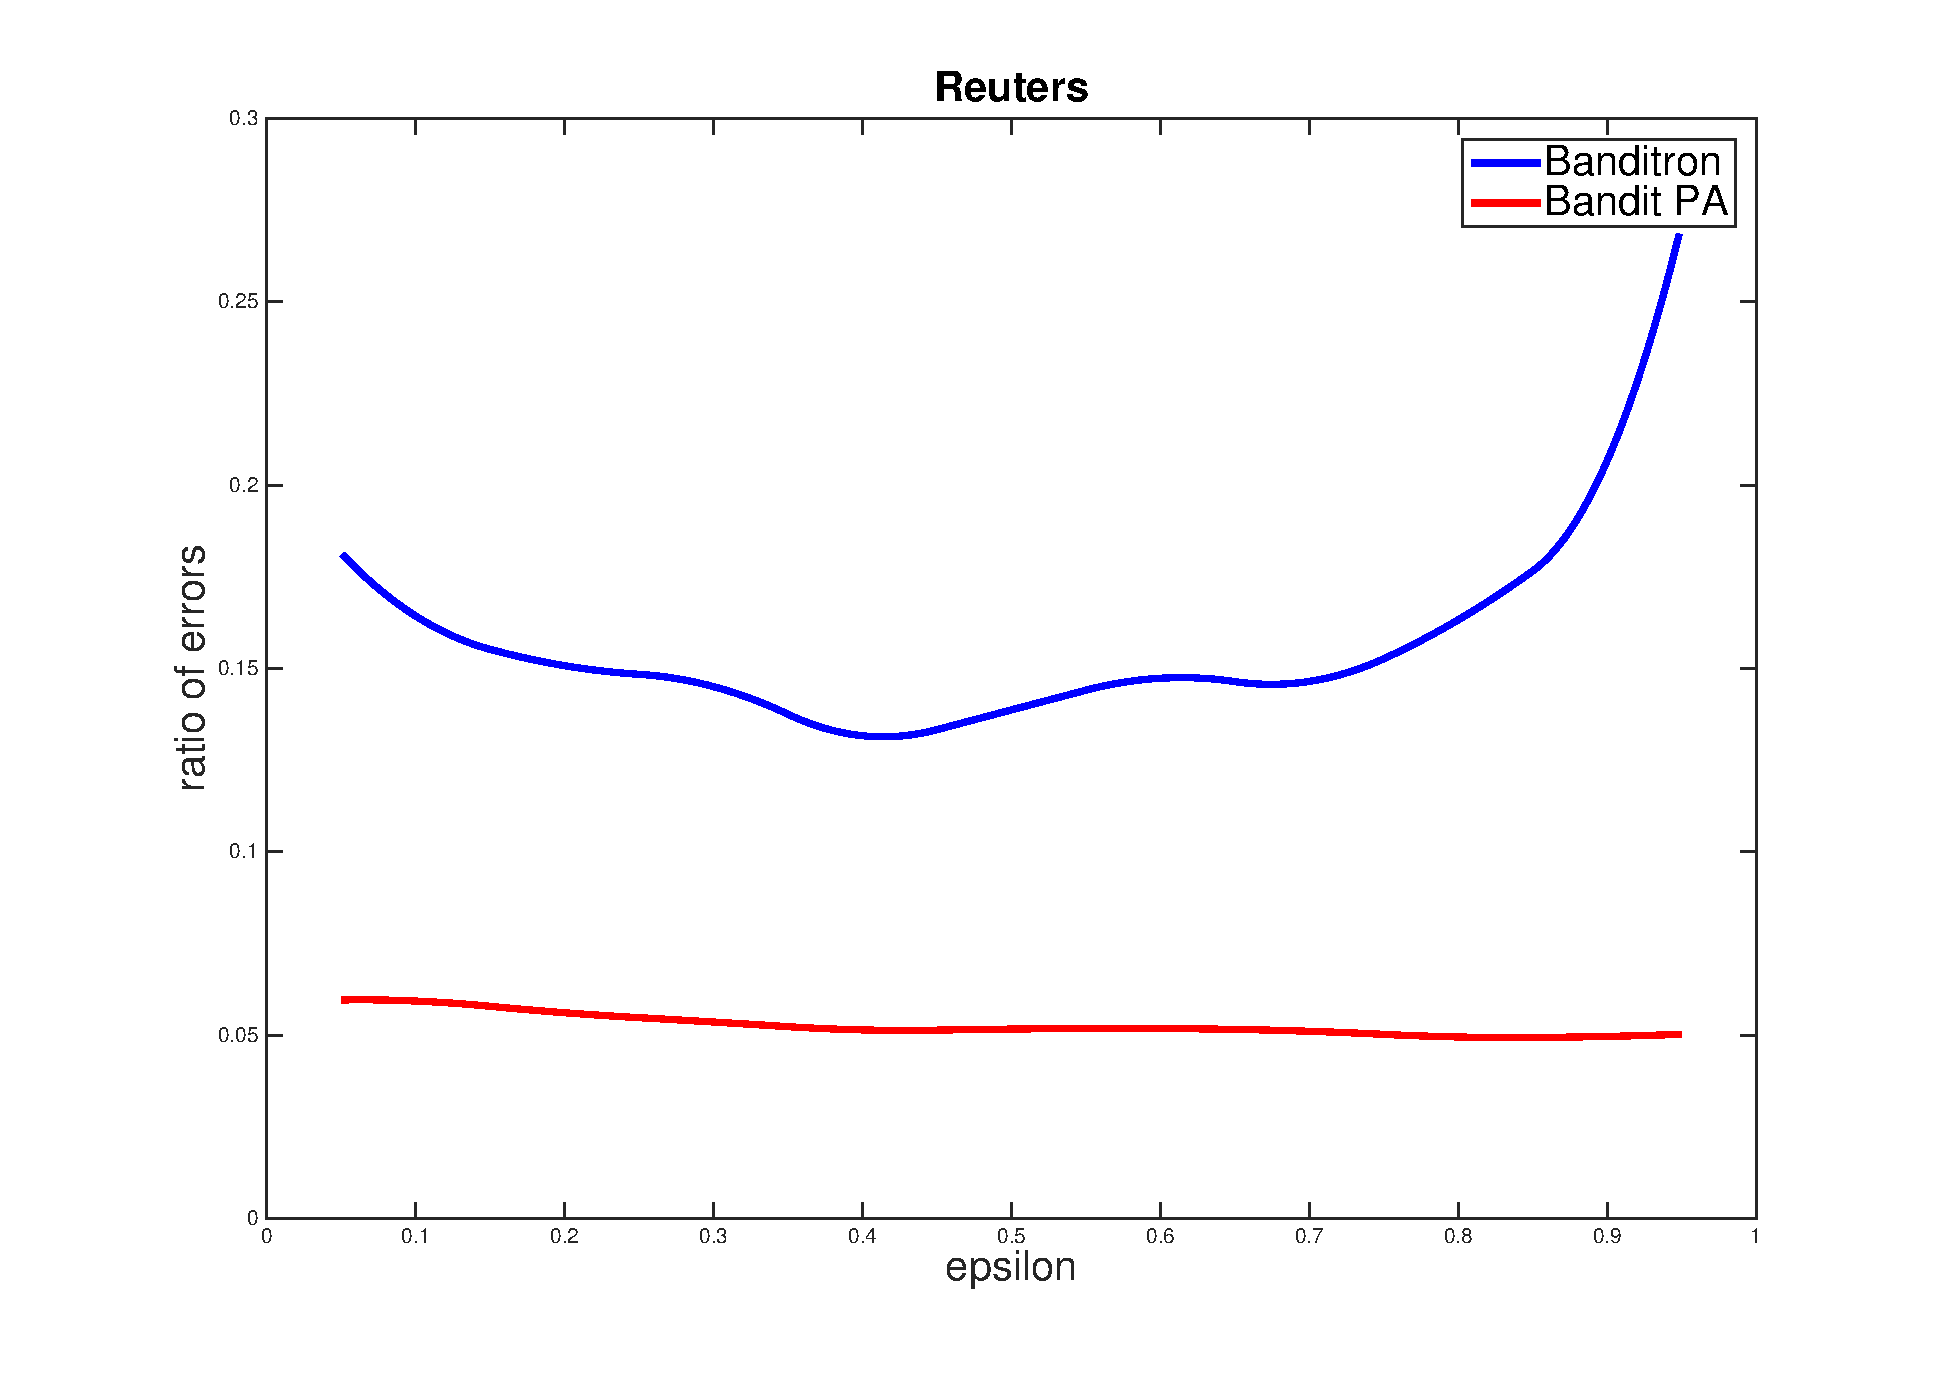
\includegraphics[width=\linewidth]{figs/Reuters_gamma.eps}}
	\caption{Taux d'erreur moyen du Banditron et du BPA en fonction du taux d'exploration $\varepsilon$ sur le jeu de données Reuters.}
	\label{pic:BPARCVerr}
\end{figure}

Les figures \ref{pic:BPASNSerr} et  \ref{pic:BPARCVerr}  présentent l'effet du paramètre d'exploration $\varepsilon$ sur les taux d'erreur obtenus en fin de session par le Banditron et le BPA, sur les bases SynNonSep et Reuters. Contrairement au Banditron, le taux de réussite du BPA est remarquablement insensible à la valeur de $\varepsilon$. Autrement dit, les performances d'apprentissage sont les mêmes pour un $\varepsilon$ faible que pour un $\varepsilon$ élevé. Ce résultat permet d'envisager la mise en place de politiques à taux d'exploration variable, afin de de profiter en fin d'apprentissage des bonnes performances du classifieur.
Par ailleurs, dans les deux cas, le taux d'erreurs obtenu par BPA en fin de session est plus faible que celui du Banditron. 


%\begin{figure}[h!]
	
%	\centerline{
%		\includegraphics[width=\linewidth]{figs/regret.eps}
%	}
%	\caption{Regret estimé sur le jeu de données Reuters pour l'algorithme BPA}
%	\label{pic:regret}
%\end{figure}

%La figure \ref{pic:regret} donne une estimation du regret cumulé sur la base Reuters pour les 20000 premiers exemplaires, pour l'algorithme BPA, en utilisant pour la comparaison le classifieur obtenu en fin de session. On observe un taux de croissance du regret cumulé sous-linéaire, compatible avec la prédiction $O(\sqrt{t})$ (voir théorème 2). 


\begin{figure}[ht!]
	
	\centerline{
		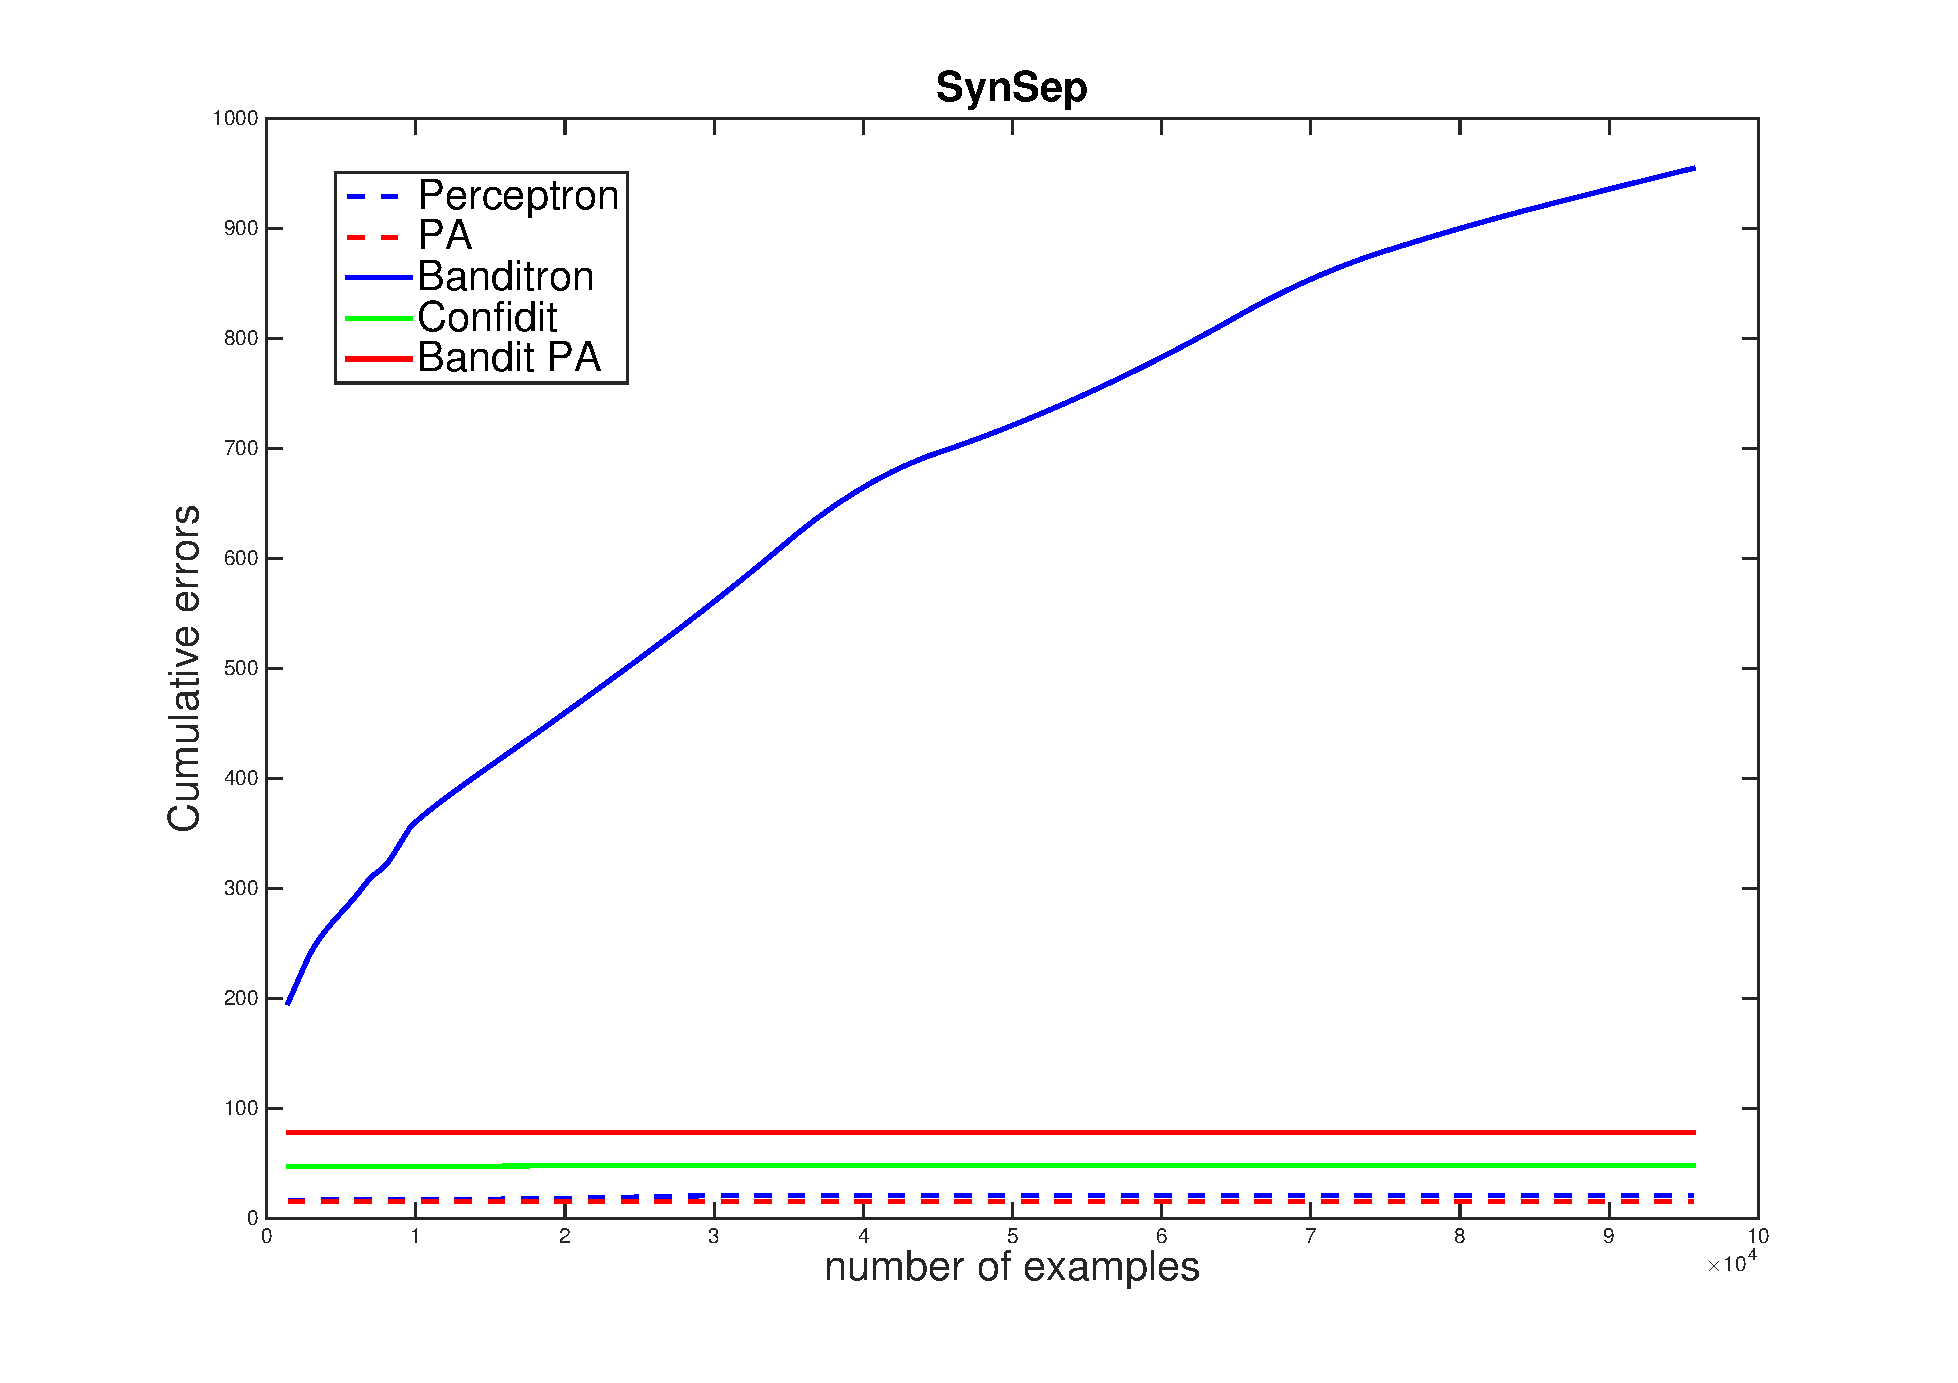
\includegraphics[width=\linewidth]{figs/SynSep.eps}
	}
	\caption{Erreurs cumulées sur le jeu de données synthétique SynSep.}
	\label{pic:BPASS}
\end{figure}
\begin{figure}[ht!]
	
	\centerline{
		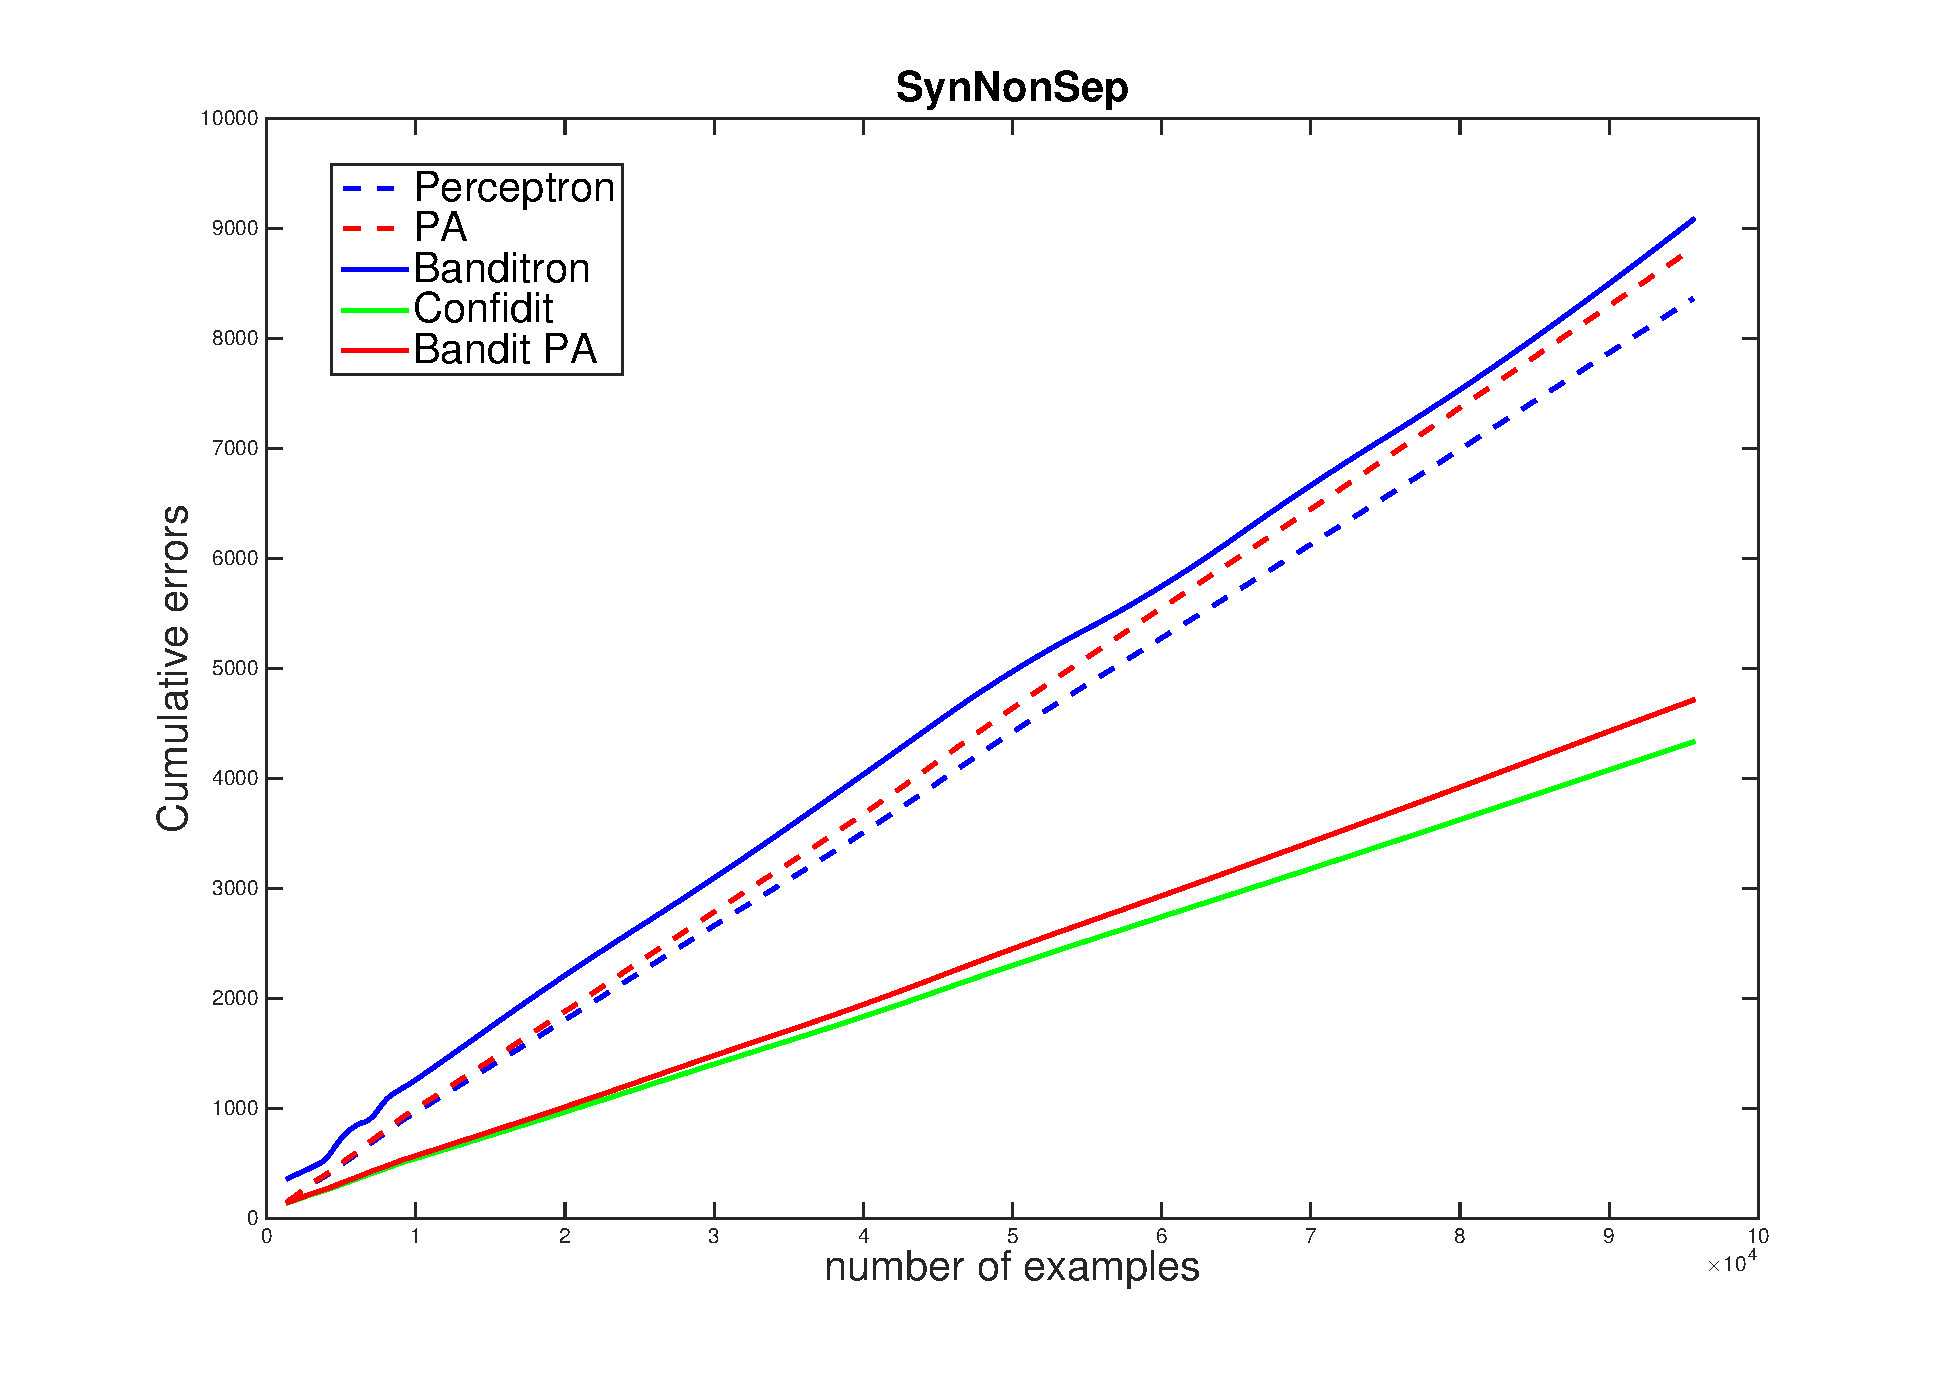
\includegraphics[width=\linewidth]{figs/SynNonSep.eps}
	}
	\caption{Erreurs cumulées sur le jeu de données synthétique SynNonSep.}
	\label{pic:BPASNS}
\end{figure}
\begin{figure}[ht!]
	\centerline{
		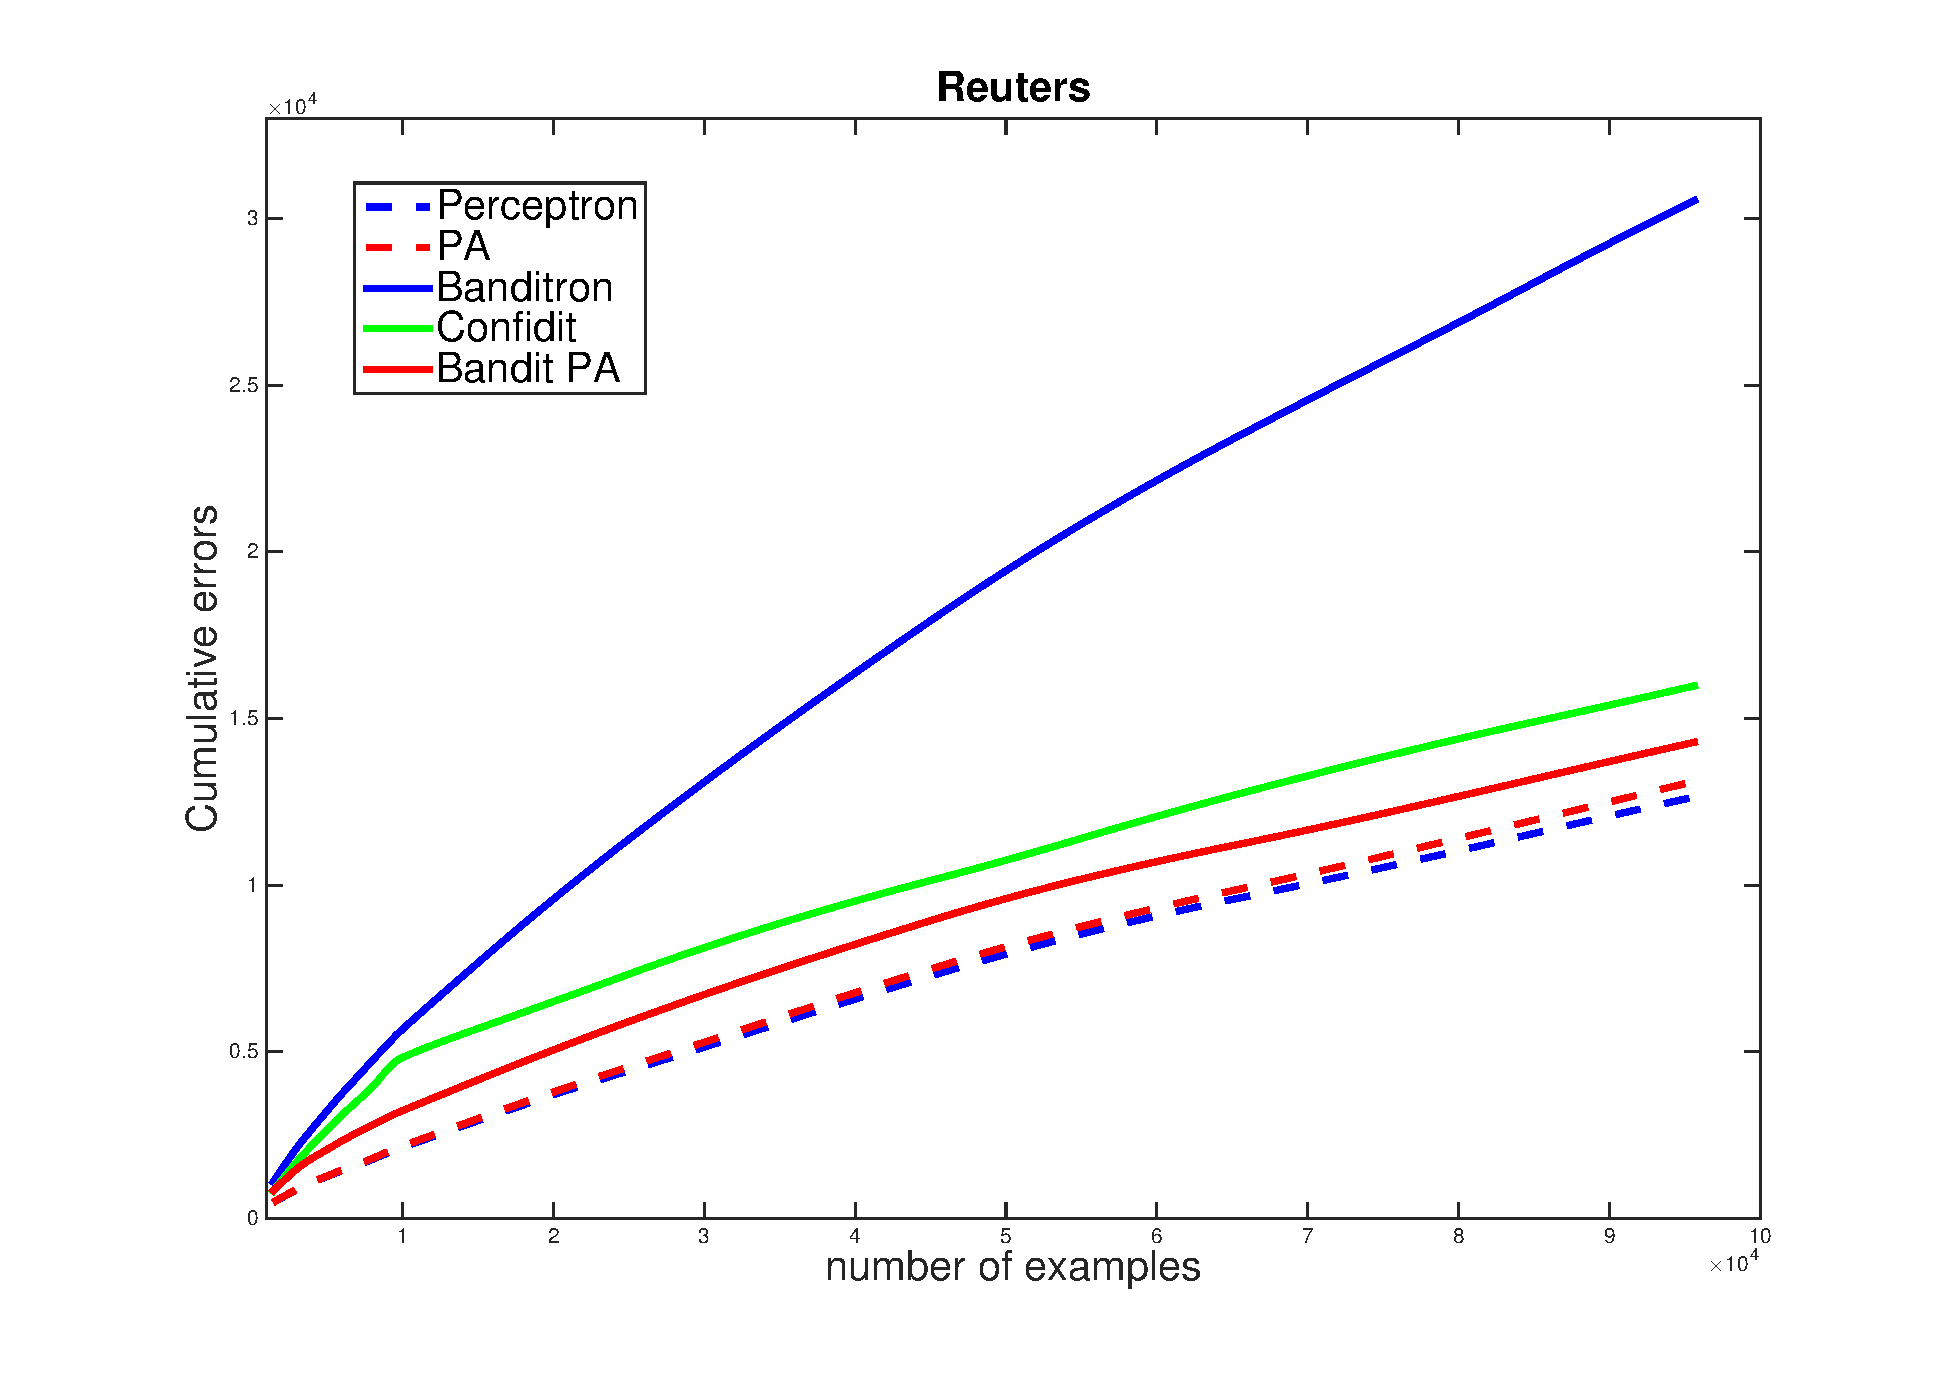
\includegraphics[width=\linewidth]{figs/RCV1_v2_53class.eps}}
	\caption{Erreurs cumulées sur le jeu de données réel RCV1-v2 (53 classes).}
	\label{pic:BPARCV}
\end{figure}

Les figures \ref{pic:BPASS}, \ref{pic:BPASNS} et \ref{pic:BPARCV} comparent les algorithmes Perceptron, Passif-Agressif (PA), Banditron, Confidit et Bandit-Passif Agressif (BPA) sur les jeux de données de grande dimension SynSep, SynNonSep, et Reuters. 

Sur le premier jeu synthétique et linéairement séparable, on constate que la borne est rapidement atteinte pour Perceptron, PA, Confidit et BPA. Seul Banditron présente une courbe croissante qui ne permet pas de borner le taux d'erreurs cumulées.  On constate également, comme prévu, un taux d'erreur total plus faible pour les algorithmes supervisés que pour les algorithmes à feedback de Bandit.

Dans le cas de SynNonSep, le taux de croissance de l'erreur cumulée est linéaire, du fait du bruit de label de 5\% qui ne permet pas de supprimer les erreurs de classification. On constate ici une plus faible sensibilité des algorithmes Confidit et BPA au bruit de label, avec une pente plus faible que pour les algorithmes supervisés.

%\textcolor{red}{OK-- Il manque les valeurs des paramètres pour les différents algorithmes (faire un tableau comme dans la partie précédente).}

Enfin, la base Reuters, qui présente le cas de figure le plus réaliste, permet de mettre en évidence les bonnes performances de l'approche BPA. Dans tous les cas, les taux d'erreurs cumulés sont croissants mais la croissance est sous linéaire, indiquant une bon comportement d'apprentissage pour tous les algorithmes. Les deux algorithmes supervisés présentent des performances comparables, avec un taux d'erreurs cumulées légèrement plus faible  que confidit et BPA, et des pentes finales à peu près comparables. Le résultat le plus saisissant ici est de constater les performances des algorithmes BPA et Confidit, très proches de celles des algorithmes supervisés malgré le nombre de classes élevé (53). Le taux d'erreurs cumulées se révèle par ailleurs un peu plus favorable pour BPA que pour Confidit, ce qui est également notable étant donnée la moindre complexité algorithmique de l'algorithme BPA \footnote{L'algorithme Confidit nécessite en effet une estimation de la covariance des échantillons, cette matrice de covariance étant réduite en haute dimension à une simple diagonale.}. Seul l'algorithme du Banditron semble encore une fois présenter une performance d'apprentissage significativement plus faible. 


Dans le cas de jeux de données de petite dimension, nous comparons le comportement des algorithmes dans le cas du plongement des données dans des espaces de fonctions noyaux. Nous notons ainsi KBanditron le Banditron à noyaux, KBPA le Bandit Passif Agressif à noyaux et KSGD l'approche basée sur la descente de gradient régularisée présenté dans la partie 2.3. Le paramètre de raideur est ici $C = \infty$, autrement dit nous considérons les données linéairement séparables dans l'espace de redescription. Nous ne présentons pas ici l'algorithme Confidit pour lequel la généralisation aux espaces de fonctions noyaux est moins directe. 

La fonction noyau utilisée dans ce cadre est la fonction de Laplace, soit~:
\[K(x,y) = \exp{\left(-\frac{\parallel{x-y}\parallel}{\sigma}\right)}\]
Les paramètres sont donnés dans la table 2. 

\begin{figure}[t!]
	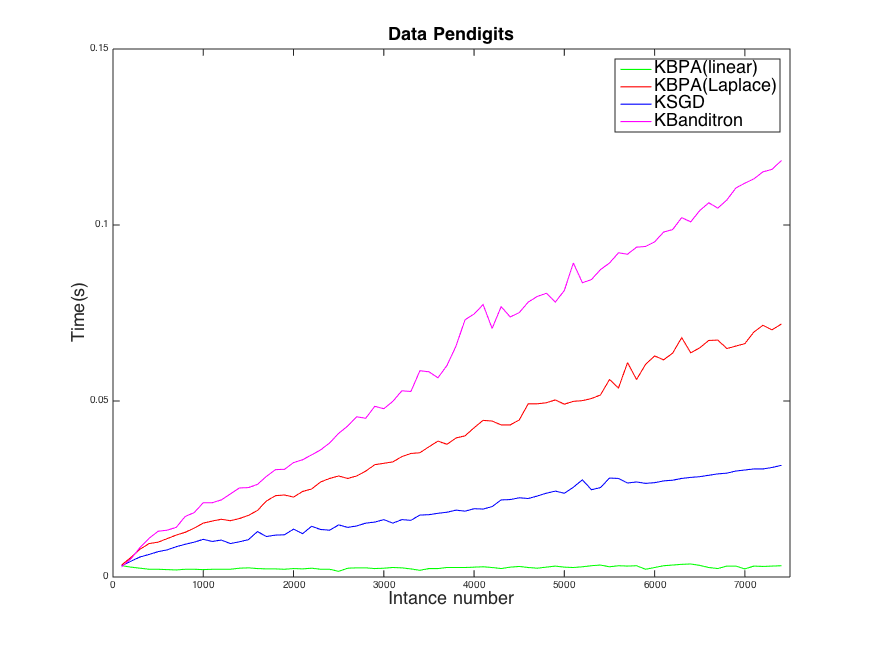
\includegraphics[width=\linewidth]{figs/Pendigits_kernel_T.png}
	\caption{Temps de simulation moyen pour le jeu de données Pendigits.}
	\label{pic:PKT}
\end{figure}

\begin{figure}[t!]
	\centerline{
		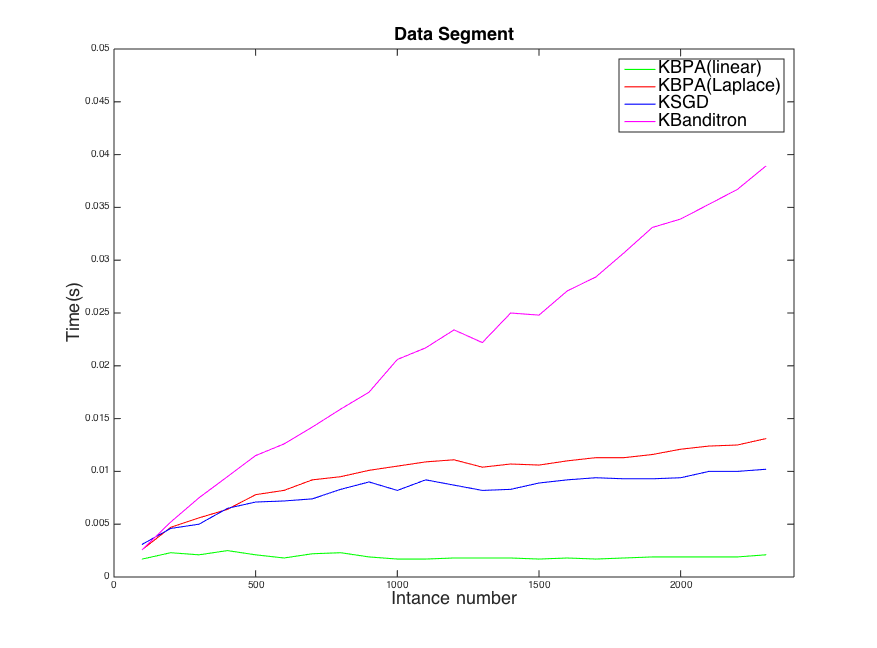
\includegraphics[width=\linewidth]{figs/Segment_kernel_T.png}}
	\caption{Temps de simulation moyen pour le jeu de données Data Segment.}
	\label{pic:SKT}
\end{figure}

Dans le cas de l'apprentissage en ligne, le nombre d'exemplaires supports des classifieurs croît au cours de l'apprentissage, ce qui tend faire croître le temps de calcul. Nous mesurons ainsi croissance du taux temps de calcul au cours de l'apprentissage pour les différents algorithmes considérés. Soit $c_t$ le temps de calcul à l'instant $t$.  Le temps de calcul moyen est calculé comme~: 
$$\forall t>99, \bar{c}_t = \frac{1}{100} \sum_{t'=t - 99}^t c_{t^\prime}$$

Les Figures~\ref{pic:PKT} et \ref{pic:SKT} présentent l'évolution du temps de calcul pour les différents algorithmes considérés sur les bases Pendigit  et Segment.  Le BPA linéaire présente comme attendu un temps de calcul indépendant du temps. On constate ensuite des temps de calcul croissants pour les trois algorithmes à noyaux. La croissance la plus forte (croissance linéaire) est observée comme attendu dans le cas du Banditron qui ajoute un exemplaire à la base des vecteurs supports à chaque nouvel essai. L'algorithme BPA présente une croissance moins marquée du nombre de vecteurs supports, du fait de la fonction de coût de type ``hinge loss'' qui permet d'ignorer les exemplaires ne produisant pas de perte.  on constate en particulier sur la base Segment une tendance à la stabilisation du temps de calcul. Enfin l'algorithme KSGD indique un temps de calcul de croissance significativement plus faible, du fait du principe de troncature utilisé. Dans le cas de la base Segments, les performances des deux algorithmes s'avèrent néanmoins très proches, indiquant la bonne parcimonie de l'algorithme BPA.

\begin{figure}[t!]
	\centerline{
		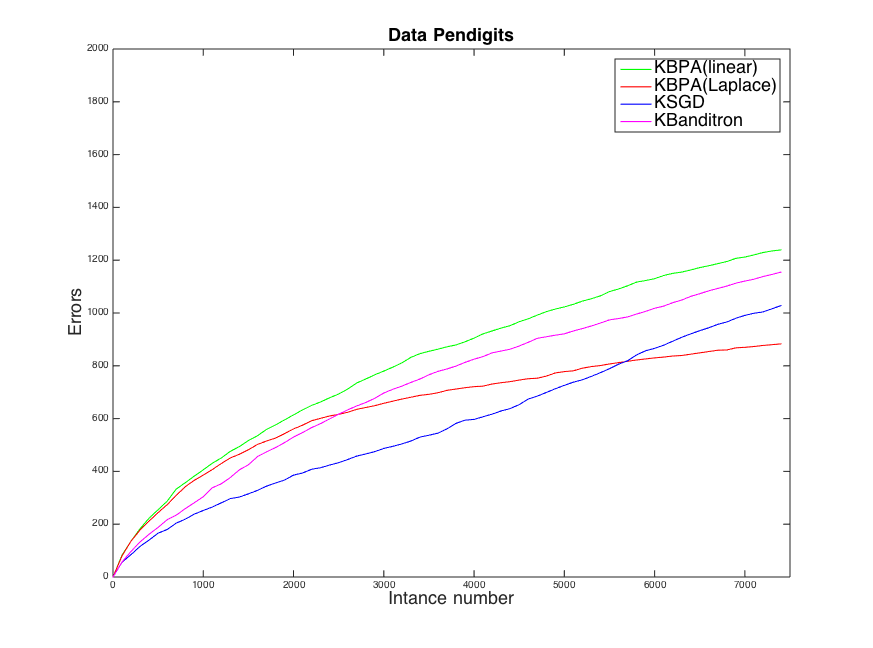
\includegraphics[width=\linewidth]{figs/Pendigits_kernel_CM.png}}
	\caption{Erreurs cumulées sur le jeu de données réelles Pendigits}
	\label{pic:PKCM}
\end{figure}

%\begin{figure}[h!]
%	\centerline{
%		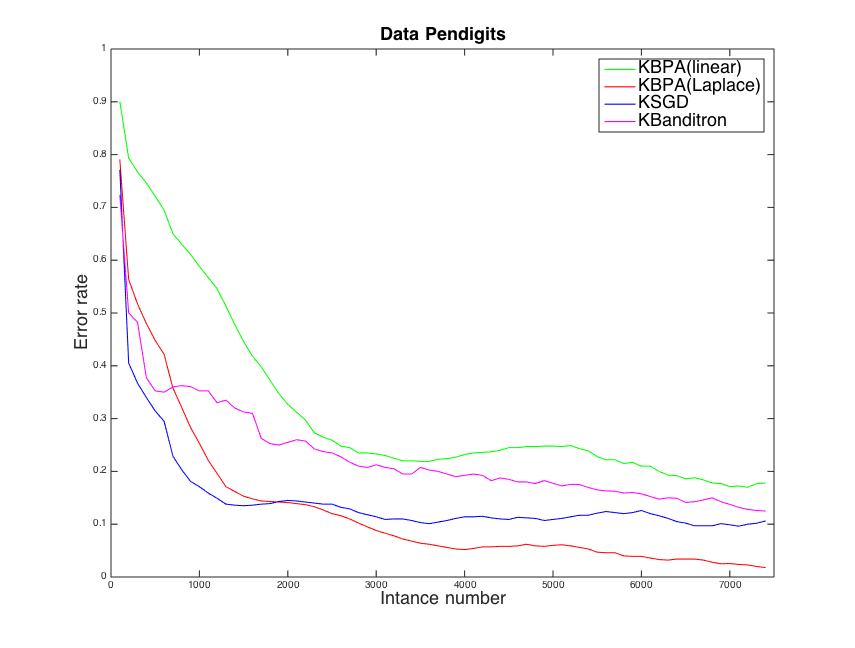
\includegraphics[width=\linewidth]{figs/Pendigits_kernel_M.png}}
%	\caption{Average error rate for each instance of Data Pendigits}
%	\label{pic:PKM}
%\end{figure}

\begin{figure}[t!]
	\centerline{
		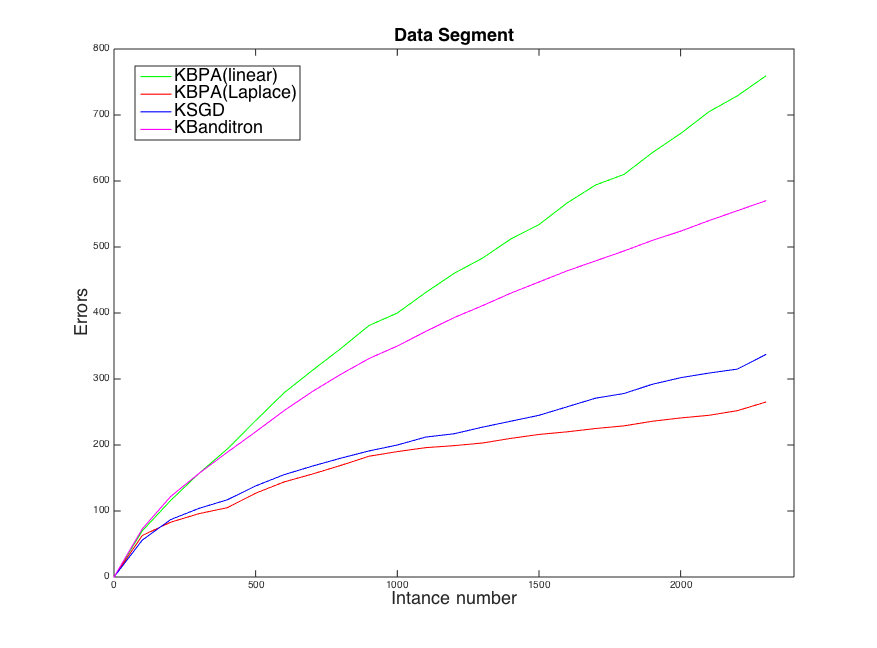
\includegraphics[width=\linewidth]{figs/Segment_kernel_CM.png}}
	\caption{Erreurs cumulées sur le jeu de données réelles Segment}
	\label{pic:SKCM}
\end{figure}

%\begin{figure}[h!]
%	\centerline{
%		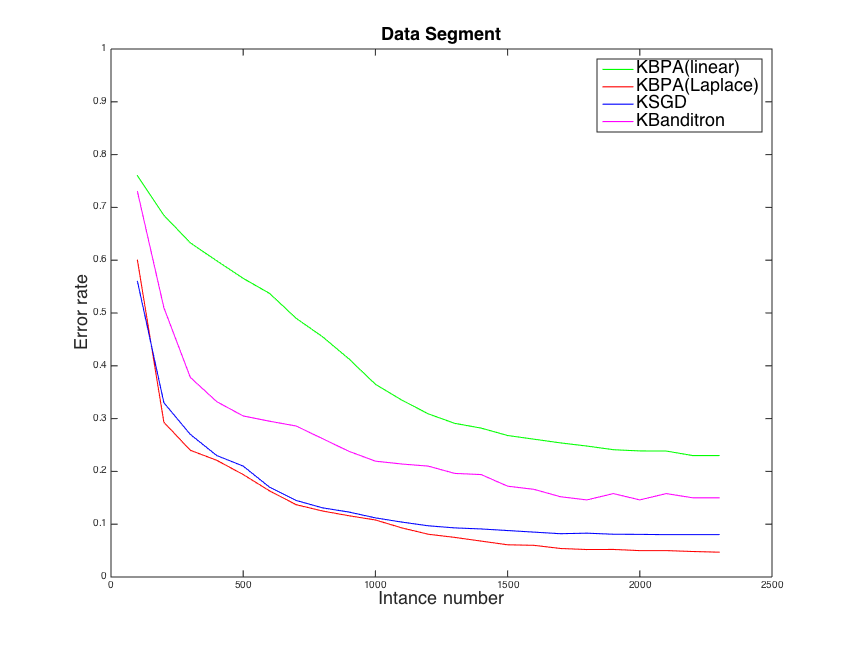
\includegraphics[width=\linewidth]{figs/Segment_kernel_M.png}}
%	\caption{Average error rate for each instance of Data Segment}
%	\label{pic:SKM}
%\end{figure}

Les figures  \ref{pic:PKCM} %, \ref{pic:PKM}, 
et \ref{pic:SKCM} 
%et \ref{pic:SKM}  
présentent enfin les taux d'erreur cumulés produits par ces différents algorithmes au cours de l'apprentissage des bases Pendigit et Segment. Les courbes d'erreurs cumulées mettent en évidence dans ce cas la supériorité de l'approche à noyaux sur l'approche linéaire, du fait du caractère non-linéairement séparable des données utilisées. Par ailleurs, l'algorithme BPA présente dans les deux cas les meilleurs performances d'apprentissage que l'algorithme du Banditron. L'algorithme KSGD présente de bonnes performances en début d'apprentissage, mais tend ensuite à atteindre un plateau de performances (du fait de la troncature) tandis que BPA présente une amélioration plus régulière lui permettant de dépasser les performances de KSGD en fin de session. On constate en particulier des taux d'erreurs très faibles en fin de session pour la base Pendigit. Ces performances d'apprentissage sont remarquables du fait de l'absence d'information de classification complète.  

%\begin{figure}[h!]
%\label{pic:PKR}
%\centerline{
%\includegraphics[scale = 0.4]{fig05/mc/Pendigits_kernel_R.png}}
%\caption{Cumulative loss of Data Pendigits}
%\end{figure}







%\begin{figure}[h!]
%\label{pic:SKR}
%\centerline{
%\includegraphics[scale = 0.4]{fig05/mc/Segment_kernel_R.png}}
%\caption{Cumulative loss of Data Segment}
%\end{figure}
%\subsection{Conclusion}
\section{Conclusion}
\label{sec:conclusion}
%{Conclusion}
%\label{subsec:BPAC}

Nous avons proposé dans cet article un nouvel algorithme d'apprentissage en ligne de classifieurs multiclasses dans le cas où l'information de classification est binaire (réponse correcte ou incorrecte). L'absence d'information de label explicite conduit à échantillonner de manière aléatoire l'espace des labels, sur le modèle des bandits contextuels. L'approche utilisée ici pour l'exploration est $\varepsilon$-glouton, soit une alternance entre échantillonnage uniforme et exploitation. 

L'algorithme développé repose  sur l'optimisation à chaque essai d'une fonction de coût spécifique, sur le modèle de l'approche ``Passive Agressive'' proposée par \cite{crammer2006online}. 
L'analyse mathématique permet de mettre en évidence des bornes sur la somme des coûts cumulés, à la fois dans le cas séparable et dans le cas non séparable, comparables aux bornes obtenues dans le cas supervisé.

Les expériences numériques confirment le bon comportement de l'algorithme d'apprentissage, à la fois sur des données de grande dimension et sur des jeux de données non-linéairement séparables. Tout en présentant une complexité algorithmique similaire, notre approche dépasse systématiquement les performances de l'algorithme du Banditron \cite{kakade2008efficient}. En particulier, nous observons une faible sensibilité au taux d'exploration $\varepsilon$, soit une conservations des performances depuis l'échantillonnage pur jusqu'à l'exploitation ``gloutonne'' de la réponse du classifieur. Cette propriété permet en conditions réelles d'envisager une implémentation de l'algorithme avec un $\varepsilon$ décroissant au cours de l'apprentissage.    

Les courbes d'apprentissage montrent des performances similaires aux méthodes d'ordre 2, tout en présentant une complexité linéaire en espace. 
Cette complexité faible permet en particulier d'appliquer aisément cette approche aux données de grande dimension. Les expériences montrent également un bon comportement dans le cas où le nombre de classes est assez élevé (ici 53 classes dans le cas de la base Reuters).  
Dans le cas où les données ne sont pas linéairement séparables, l'algorithme présente une bonne parcimonie, permettant d'éviter une croissance trop importante du nombre de vecteurs supports au cours de l'apprentissage.

Plus généralement, ces résultats illustrent le fait qu'une information de classification minimale (ici binaire) se révèle suffisante pour un apprentissage multi-classes performant, offrant en particulier des bornes de convergence comparable en ordre de grandeur à celles reposant sur une information de classification complète.


\bibliography{cap2016}

\end{document}

%%% Local Variables: 
%%% mode: latex
%%% TeX-master: t
%%% End: 
